

\chapter{Aufgabenblatt 05}

\section{ User Experience and Usability }
Das  von  Ihrer  IT  Abteilung  zu  entwickelnde  mobile  Universit"ats-Portal  dient  vorwiegend  der Nutzung  durch  Studenten.  
Jedoch  auch  f"ur  die  Bediensteten  der  Hochschule  bieten  sich dadurch  zahlreiche  Vorteile.  
In  der  Vorlesung  haben  Sie  Methoden  des  Prototyping, Storytelling sowie die Erstellung von Personas kennengelernt. 


\subsection{Aufgabe 1: Personas}
Im  Rahmen  der  Usability  Methoden  haben  Sie  neben  der  Nutzergruppendefinition  das Konstrukt der Personas kennengelernt.  
Bitte erstellen Sie insgesamt vier Personas, davon jeweils zwei f"ur die Gruppe der Studenten sowie zwei f"ur die Gruppe der Bediensteten. 

\textbf{L"osung:}
\begin{itemize}
    \item Student 1 : Max Mustermann\\
        M"annlich, studiert im 3. Semester Maschinenbau.
        Mag vornehmlich fleischlastige und deftige Speisen, m"ochte schnell und g"unstig in seiner Mittagspause etwas essen.
        Hat nicht den Willen, beim Essen am Handy zu sein und w"ahrenddessen sozial zu interagieren.
        Das Essen ist f"ur ihn eher Mittel zum Zweck als eine T"atigkeit, mit der er sich auseinander setzt.
    \item Student 2 : Martina Mustermann\\
        Weiblich, studiert im 5. Semester Gender Studies.
        Vegan aus "Uberzeugung, w"ahlt ihr Essen bewusst aus und setzt sich intensiv mit ihrer Nahrungsaufnahme auseinander.
        Interagiert st"andig sozial, bewertet gerne Produkte online und schreibt Rezensionen.
    \item Bediensteter 1: Jon Doe\\
        Wie Max, ist blo"s schon fertig mit seiner Ausbildung und 40 Jahre alt. 
    \item Bediensteter 2 : Jennifer Doe\\
        Wie Martina, abgesehen von der Tatsache dass sie 45 Jahre alt ist und mit ihrer Ausbildung fertig.
\end{itemize}

\subsection{Aufgabe 2:  Contextual Inquiry and Storytelling }
Um  die  Bed"urfnisse  der  Nutzer  bestm"oglich  abzudecken  und  damit  eine  erfolgreiche Anwendung zu erstellen ist es unabdingbar, den sp"ateren Nutzungskontext zu kennen.\\
\begin {enumerate}
    \item Bitte beschreiben Sie exemplarisch (2-3 S"atze) den Nutzungskontext f"ur jede der zuvor erstellten  Personas.  
        F"ur  die  Gruppe  der  Studenten  soll  dabei  ein  Interview  mit Kommilitonen dienen, die in der jeweiligen Nutzergruppe liegen.  \\
    \textbf{L"osung:}
    \begin{itemize}
        \item Max: \\
            Er geht in die Mensa mit dem Ziel, schnell satt zu werden und wieder herauszukommen.
            Er m"ochte schnell und g"unstig etwas essen.
            Er hat nicht vor, die App f"ur soziale Interaktion zu nutzen.
        \item Martina: \\
            Sie geht in die Mensa mit dem Ziel, etwas gesundes und "okologisch wertvolles zu essen.
            Sie nimmt sich Zeit zum essen und zahlt auch gerne etwas mehr, falls das Essen ihren Qualit"atsanspr"uchen gen"ugt.
            Sie will die App zum bewerten von Gerichten und zum sozial interagieren verwenden.
        \item Jon: \\
            Wie Max,nur "alter und mit etwas mehr Budget.
        \item Jennifer: \\
            Wie Martina, nur mit mehr Zeit, ausf"uhrlicheren Bewertungen und noch h"oheren Qualit"atsanspr"uchen.
    \end{itemize}
    \item W"ahlen  Sie  zwei  der  erstellten  Personas  aus  und  wenden  Sie  die  Methode  des Storytelling  an.  
        Wie  kann  die  sp"atere  Nutzung  des  Mensa  Moduls  anhand  einer Geschichte erz"ahlt werden? \\
    \textbf{L"osung:}        
    \begin{itemize}
        \item Max: \\
            Max m"ochte in der app schnell die im Moment g"unstigste Mensa finden, die f"ur ihn am schnellsten zu erreichen ist. 
            Hierf"ur sieht er sich zuerst die Mensa- "Ubersicht an und dann die jeweiligen Speisepl"ane. 
            Hat er dies erledigt, benutzt er die App, um sich zur Mensa seiner Wahl navigieren zu lassen. 

        \item Martina: \\
            Martina nutzt die app ausgiebig, um sich "uber die Zutaten der einzelnen Gerichte zu informieren und so das ihr am besten gefallende Gericht zu finden. 
            Sobald sie ein Gericht ausgesucht hat, l"asst sie sich zur entsprechenden Mensa navigieren.
            Beim Essen tauscht sie sich "uber die Community- Features der app mit anderen, in der Mensa anwesenden Personen "uber das Gericht, welches sie gerade isst, aus.
            Sobald sie mit dem Essen fertig ist, verfasst sie eine Rezension und ein gibt ein Rating f"ur das Gericht ab.
    \end{itemize}
\end {enumerate}

\subsection{Aufgabe 3: Prototyping  }
Das  Prototyping  einer  Anwendung  dient  unter  anderem  der  fr"uhzeitigen  Visualisierung  der sp"ateren Anwendung. 
Um Ihr Konzept so bald wie m"oglich anhand der Nutzergruppe validieren zu können entschlie"sen Sie sich, das Mensa Modul als Mockup umzusetzen.  
Erstellen  Sie  dazu  Design- Mockups  
\begin {itemize}
    \item Der  Mensa  Startseite, des Speiseplans\\
    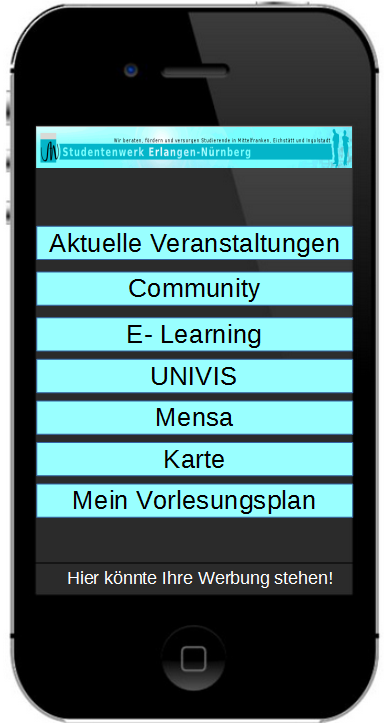
\includegraphics[scale=0.4]{./inc/aufgabe05/MockupStartseite} 
    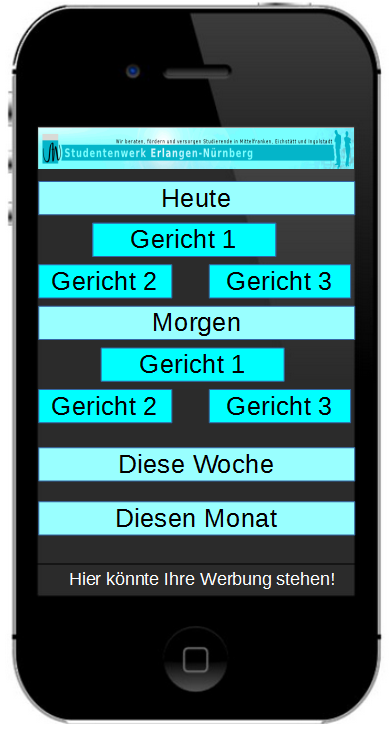
\includegraphics[scale=0.4]{./inc/aufgabe05/MockupSpeiseplan}
    \item und der Detailseite eines Gerichts inklusive Bewertungssystem.\\ 
    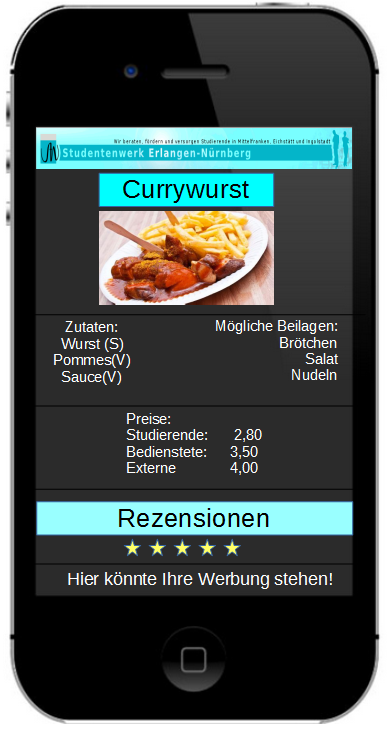
\includegraphics[scale=0.4]{./inc/aufgabe05/MockupGericht}
\end{itemize}
        

    
